% !TEX program = xelatex
% 基于卷积神经网络的图像分类 —— 实验报告（XeLaTeX 版）
% 编译：xelatex report.tex 两次（交叉引用与总页数需要第二次），或运行 build_tex.py
\documentclass[10.5pt,a4paper,UTF8]{article}

% ------------------------------------------------------------------ 页面
\usepackage[a4paper,top=1.5cm,bottom=1.4cm,left=1.55cm,right=1.55cm]{geometry}
\usepackage{fontspec}
\usepackage[heading=true,fontset=none]{ctex}
\usepackage{graphicx}
\usepackage{array,tabularx,ragged2e}
\setlength{\RaggedRightParindent}{2em}
\usepackage{booktabs}
\usepackage{makecell}
\usepackage{caption}
\usepackage{xcolor}
\usepackage{enumitem}
\usepackage{amsmath}
\usepackage{fancyhdr}
\usepackage[colorlinks=true,linkcolor=blue!55!black,urlcolor=blue!55!black]{hyperref}
\usepackage{indentfirst}

% ------------------------------------------------------------------ 字体
\setmainfont{Times New Roman}
\setCJKmainfont{SimSun}[BoldFont=SimHei]
\setCJKsansfont{SimHei}
\newcommand{\code}[1]{{\ttfamily\small #1}}
\newCJKfontfamily\heiti{SimHei}

% ------------------------------------------------------------------ 版式
\linespread{1.0}
\setlength{\parindent}{2em}
\setlength{\parskip}{0pt}
\setlength{\emergencystretch}{2em}
\captionsetup{font=small,labelsep=quad,skip=2pt}
\renewcommand{\figurename}{图}
\renewcommand{\tablename}{表}
\setlist[enumerate]{leftmargin=1.5em,itemsep=1pt,topsep=2pt,parsep=0pt}
\setlist[enumerate,1]{leftmargin=0pt,labelindent=0pt,labelwidth=1.5em,labelsep=0pt,align=left,itemindent=1.5em}
\pagestyle{fancy}
\fancyhf{}
\fancyfoot[C]{\small \thepage}
\renewcommand{\headrulewidth}{0pt}
\setlength{\textfloatsep}{8pt plus 2pt minus 2pt}
\setlength{\floatsep}{6pt plus 1pt minus 1pt}
\setlength{\intextsep}{6pt plus 1pt minus 1pt}
\ctexset{
  section = {format = \heiti\large\raggedright, beforeskip = 5pt,
             afterskip = 2pt, aftername = \quad},
  subsection = {format = \heiti\normalsize\raggedright,
                beforeskip = 4pt, afterskip = 1pt, aftername = \quad},
}
\newcolumntype{L}[1]{>{\raggedright\arraybackslash}p{#1}}
\newcolumntype{Q}[1]{>{\centering\arraybackslash}p{#1}}
\newcommand{\hl}[1]{\textbf{#1}}
\newcommand{\thd}[1]{\textbf{#1}}

\begin{document}

% ------------------------------------------------------------------ 标题
\begin{center}
  {\heiti\LARGE 基于卷积网络的图像分类 实验报告}\\[3pt]
  {\small 姓名：成员 A、成员 B\quad 学号：0000000000、0000000000}
\end{center}
\vspace{-6pt}
\hrule
\vspace{1pt}

% ------------------------------------------------------------------ 1
\section{实验设置与总体流程}
实验全部在自建的统一训练框架中完成。原版的
\code{resnet-cifar100.py} 与 \code{config.yml} 没有改动。
为便于比较，除专门考察的变量外，各项实验都固定 seed=42、开启 AMP 混合精度，
CIFAR-100 用 batch=256，交通标志用 batch=64，SGD 的 momentum 与 weight decay
分别取 0.9 与 $10^{-4}$。每组实验逐 epoch 记录训练损失、测试精度、耗时与学习率，
写入 \code{results/*.csv}，同时保存最佳权重，图表与本文的数据都直接读自这些文件。
环境信息见表~\ref{tab:setup}。

\begin{table}[h]
\centering
\caption{实验环境与统一设置}\label{tab:setup}
\small
\begin{tabular}{@{}L{2.6cm}L{13.2cm}@{}}
\toprule
\thd{项目} & \thd{配置}\\
\midrule
数据集 & CIFAR-100：100 类，50000 训练 / 10000 测试，32$\times$32；\\
       & 交通标志：10 类，6024 训练 / 324 测试，原始 224$\times$224（训练时缩放）\\
软件环境 & Python 3.12、PyTorch 2.11.0+cu128、torchvision 0.26.0、CUDA 12.8\\
硬件 & NVIDIA RTX 4070 Laptop（8\,GB）\\
统一设置 & seed=42；AMP 混合精度；CIFAR batch=256、交通标志 batch=64；\\
       & SGD momentum=0.9、weight decay=$10^{-4}$（另做 Adam/AdamW/RMSprop 对比）\\
\bottomrule
\end{tabular}
\end{table}

% ------------------------------------------------------------------ 2
\section{任务 1：跑通 ResNet10 + CIFAR-100 基线}
\subsection{完成过程}
装好 \code{requirements.txt} 中的 PyTorch、torchvision 与 ignite，确认 CUDA 可用后，
直接运行 \code{resnet-cifar100.py}（\code{config.yml}：SGD、lr=0.001、batch=256、50 epoch），
完整训练 50 个 epoch，最佳精度 37.21\%，总耗时 13.1 min。原版脚本与配置文件都没有改动。

\begin{table}[h]
\centering
\caption{原版脚本的运行结果}\label{tab:t1}
\small
\begin{tabular}{@{}L{3.0cm}L{2.6cm}*{3}{>{\centering\arraybackslash}p{1.8cm}}@{}}
\toprule
\thd{脚本} & \thd{优化器 / lr} & \thd{epoch} & \thd{最佳精度(\%)} & \thd{耗时(min)}\\
\midrule
\code{resnet-cifar100.py} & SGD / 0.001 & 50 & \hl{37.21} & 13.1\\
\bottomrule
\end{tabular}
\end{table}

\subsection{结果分析}
37.21\% 说明网络、数据加载与训练流程可以正常完成一轮完整训练。
日志中训练损失到第 50 epoch 仍有 2.34，末轮精度低于中途的最好值，
对应 \code{config.yml} 中的学习率 0.001：该学习率下 SGD 在 50 epoch 内尚未收敛。

% ------------------------------------------------------------------ 3
\section{任务 2：优化器对比（SGD / Adam / AdamW / RMSprop）}
\subsection{完成过程}
固定 ResNet10、batch=256、50 epoch 与恒定学习率，只替换优化器，分别用 SGD(lr=0.1)、
Adam($10^{-3}$)、AdamW($10^{-3}$)、RMSprop($10^{-3}$)，动量与权重衰减保持一致，结果见表~\ref{tab:opt}
与图~\ref{fig:optim}。

\begin{table}[h]
\centering
\caption{四种优化器对比（ResNet10、CIFAR-100、恒定 lr、50 epoch）}\label{tab:opt}
\small
\begin{tabular}{@{}L{4.4cm}Q{1.5cm}Q{1.8cm}Q{1.8cm}Q{1.7cm}@{}}
\toprule
\thd{优化器} & \thd{lr} & \makecell{\thd{最佳}\\\thd{精度(\%)}} & \makecell{\thd{末轮}\\\thd{精度(\%)}} & \makecell{\thd{耗时}\\\thd{(min)}}\\
\midrule
SGD (momentum=0.9) & 0.1 & 66.44 & 64.85 & 6.5\\
Adam & 0.001 & 66.16 & 65.28 & 6.5\\
AdamW & 0.001 & \hl{66.70} & 66.29 & 6.5\\
RMSprop (momentum=0.9) & 0.001 & 51.70 & 48.27 & 6.6\\
\bottomrule
\end{tabular}
\end{table}

\begin{figure}[h]
  \centering
  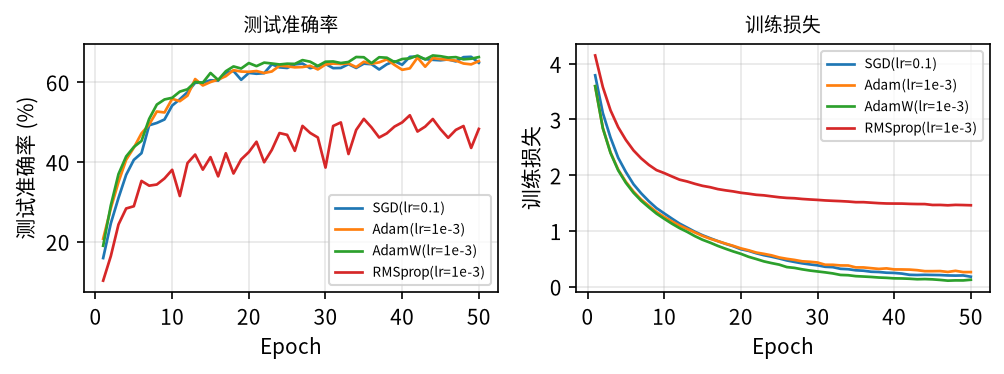
\includegraphics[width=0.8\textwidth]{../results/figs/fig1_optim.png}
  \caption{四种优化器的测试准确率与训练损失（ResNet10，CIFAR-100，50 epoch，恒定 lr）}\label{fig:optim}
\end{figure}

\subsection{结果分析}
前 20 个 epoch 中 Adam 与 AdamW 的精度上升最快，Adam 第 20 epoch 为 62.60\%，SGD 同期约 62\%，
二十个 epoch 之后三条曲线基本重合。最终 AdamW 66.70\%、SGD 66.44\%、Adam 66.16\%，
最大差距 0.54 点；在学习率各自合适的情况下，三者最终精度差别有限。
AdamW 略高，但需要额外调参，实验中 SGD 加动量已能得到接近的结果。

RMSprop 为 51.70\%，训练损失在后期停在 1.46 左右不再下降，
测试精度在 44\%$\sim$52\% 之间波动，属于 lr=$10^{-3}$ 下 50 epoch 未收敛的情形；
受实验时间限制，未再调整其学习率。

作为对照，同为 SGD 只把恒定 lr 换成 step 衰减，精度从 66.44\% 升到 71.38\%，提高 4.94 点，
大于更换优化器带来的差距。

% ------------------------------------------------------------------ 4
\section{任务 3：学习率影响与动态调节}
\subsection{完成过程}
先在 SGD 下做固定学习率扫描，取 lr = 0.001 / 0.01 / 0.1 / 0.3，其余设置完全相同，各训练 50 epoch，
其中 lr=0.001 就是任务 1 原版脚本的配置，0.1 与任务 2 的 SGD 组是同一次训练，结果见表~\ref{tab:lr}
与图~\ref{fig:lr}。随后做动态调节：以 0.1 为初值，在第 30、40 epoch 各降 10 倍
（$0.1\rightarrow0.01\rightarrow0.001$），记录训练损失随 epoch 的曲线和对应精度，见图~\ref{fig:decay}。

\begin{table}[h]
\centering
\caption{不同恒定学习率下的精度对比（SGD、ResNet10、50 epoch）}\label{tab:lr}
\small
\begin{tabular}{@{}L{3.2cm}Q{1.4cm}Q{1.4cm}Q{1.4cm}Q{1.4cm}@{}}
\toprule
SGD 学习率（恒定） & 0.001 & 0.01 & 0.1 & 0.3\\
\midrule
最佳精度(\%) & 36.86 & 63.60 & \hl{66.44} & 63.47\\
末轮精度(\%) & 36.16 & 61.61 & 64.85 & 61.22\\
\bottomrule
\end{tabular}
\end{table}

\begin{figure}[h]
  \centering
  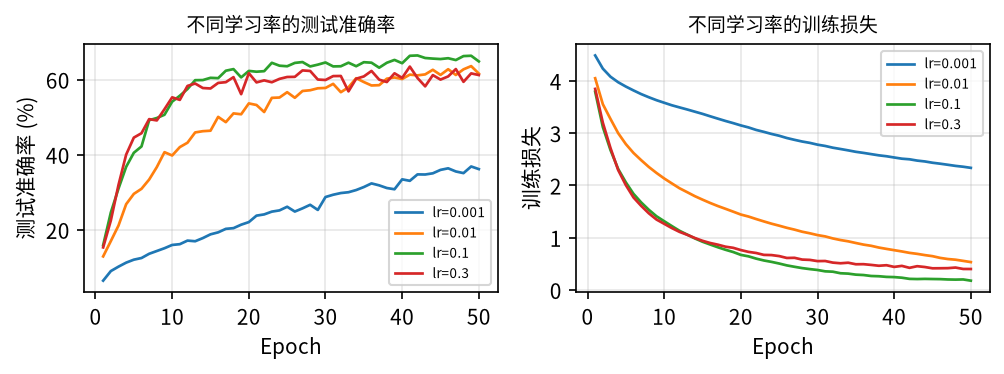
\includegraphics[width=0.8\textwidth]{../results/figs/fig2_lr.png}
  \caption{不同学习率下的测试准确率与训练损失（SGD，ResNet10，恒定 lr，50 epoch）}\label{fig:lr}
\end{figure}

\subsection{结果分析}
精度随学习率呈 U 形变化。lr=0.001 时只有 36.9\%，训练损失 2.34 且到末轮仍在下降，属于欠拟合；
0.01 为 63.6\%；0.1 最高，66.4\%；0.3 回落到 63.5\%。
lr=0.3 的末轮训练损失 0.400 高于 0.1 的 0.177，测试精度在后 20 epoch
于 58\%$\sim$63\% 之间波动，对应步长过大时在极小值附近震荡的情形。

第 30 到 31 epoch 学习率由 0.1 降到 0.01，精度由 65.40\% 升到 70.73\%，提高 5.33 点；
第 40 epoch 再降一次后趋于稳定，最佳 71.38\% 出现在第 45 epoch，比恒定 0.1 高 4.94 点。
训练损失呈台阶式下降：第 30 epoch 末约 0.38，降 lr 后为 0.21，第 40 epoch 末 0.09，最终 0.080，曲线波动很小。
这与前面的扫描一致：前期需要较大步长，后期需要较小步长，一次训练中兼顾两者需借助调度。
任务 6 因此改用余弦退火。

\begin{figure}[h]
  \centering
  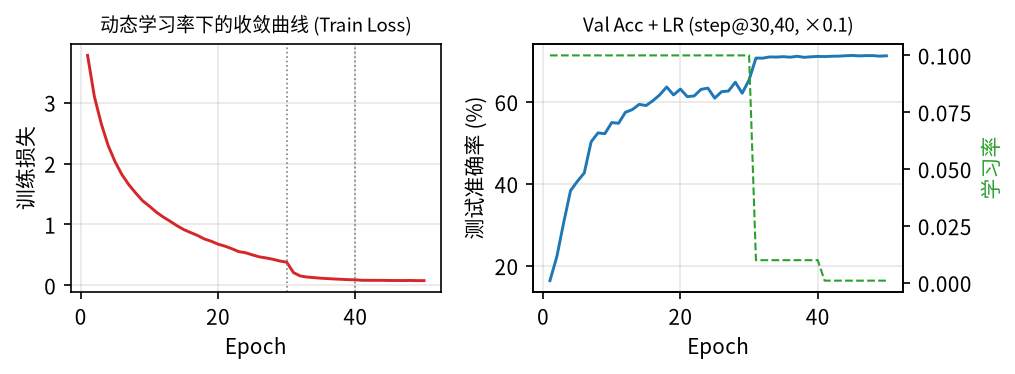
\includegraphics[width=0.8\textwidth]{../results/figs/fig3_decay.png}
  \caption{学习率动态衰减（第 30、40 epoch 各降 10 倍）下的训练损失与测试精度收敛曲线}\label{fig:decay}
\end{figure}

% ------------------------------------------------------------------ 5
\section{任务 4：网络改为 ResNet18 / ResNet50 并对比三种网络}
\subsection{完成过程}
原版代码只能构造 ResNet10，这里把构造方式改成可以传入 block 类型与各 stage 层数，
从而得到 ResNet18（BasicBlock，[2,2,2,2]）与 ResNet50（Bottleneck，[3,4,6,3]）。
分类头维度按 $512\times$expansion 自动计算，ResNet50 即为 2048。
三种网络沿用同一套为 CIFAR 设计的 stem（$3\times3$ 卷积、去掉 maxpool、只下采样三次），
训练配置也完全一致（SGD lr=0.1 加 step 衰减、50 epoch、batch=256、AMP），只改网络本身。
ResNet50 训练中途因为显存和内存压力中断过一次，从最佳权重热启动补看了剩余 epoch，
学习率按同样的调度恢复。三种网络的规模、耗时与精度见表~\ref{tab:arch} 与图~\ref{fig:arch}。

\begin{table}[h]
\centering
\caption{ResNet10 / 18 / 50 的规模、耗时与精度（CIFAR-100）}\label{tab:arch}
\small
\begin{tabular}{@{}L{2.2cm}L{3.8cm}Q{1.5cm}Q{1.4cm}Q{1.4cm}Q{1.4cm}@{}}
\toprule
\thd{网络} & \thd{结构} & \makecell{\thd{参数量}} & \makecell{\thd{总耗时}\\\thd{(min)}} & \makecell{\thd{每 epoch}\\\thd{(min)}} & \makecell{\thd{最佳}\\\thd{精度(\%)}}\\
\midrule
ResNet10 & BasicBlock [1,1,1,1] & 4,949,412 & 6.5 & 0.12 & 71.38\\
ResNet18 & BasicBlock [2,2,2,2] & 11,220,132 & 12.6 & 0.22 & \hl{72.73}\\
ResNet50 & Bottleneck [3,4,6,3] & 23,705,252 & 45.1 & 0.96 & 70.16\\
\bottomrule
\end{tabular}
\end{table}

\begin{figure}[h]
  \centering
  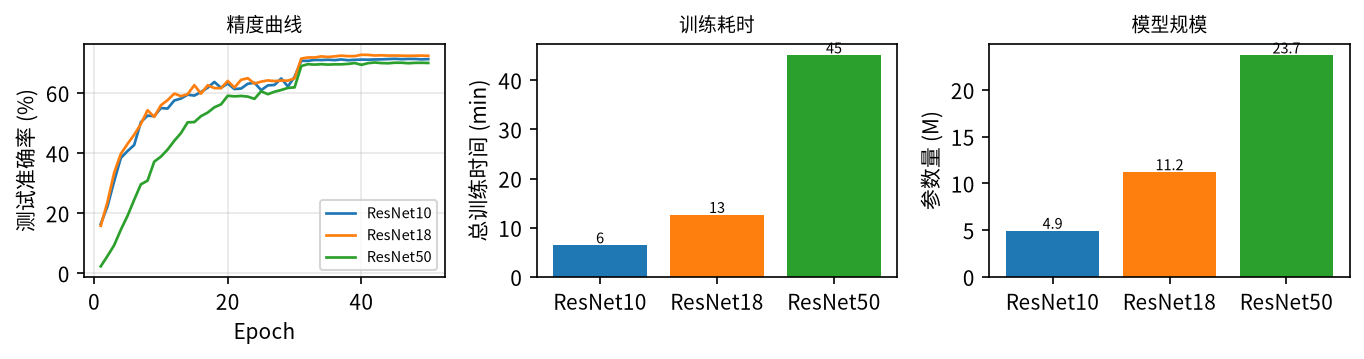
\includegraphics[width=0.95\textwidth]{../results/figs/fig4_arch.png}
  \caption{ResNet10/18/50 的精度曲线、训练耗时与参数量对比}\label{fig:arch}
\end{figure}

\subsection{结果分析}
精度没有随深度单调上升。ResNet10 为 71.38\%，ResNet18 升到 72.73\%（+1.35 点），
ResNet50 降到 70.16\%（$-2.57$ 点）。训练开销随之增加：总耗时 6.5、12.6、45.1 min，
ResNet50 参数量 23.7\,M，是 ResNet18 的 2.1 倍，单 epoch 时间大约是它的 4.3 倍
（0.22 对 0.96 min）。

ResNet50 的末轮训练损失为 0.105，高于 ResNet18 的 0.034，训练损失仍在下降区间，
属于 50 epoch 预算内尚未收敛，而非过拟合。32$\times$32 的输入下，参数量更大的模型优化更慢，
短预算内难以体现容量优势。三项中 ResNet18 精度最高、耗时居中（72.73\%，12.6 min），
任务 5 因此选它作学生网络。



% ------------------------------------------------------------------ 6
\section{任务 5：知识蒸馏（ResNet50 教师 $\rightarrow$ ResNet18 学生）}
\subsection{完成过程}
教师直接用任务 4 训练好的 ResNet50 最佳权重（最佳精度 70.16\%，第 42 epoch），推理模式下不更新参数。
学生仍为 ResNet18，训练配置与任务 4 的无蒸馏基线完全一致，只把损失函数换掉，
这样结果的差异只能归因于蒸馏。

两种损失都实现了。第一种是 Hinton 提出的 soft target，温度 $T=4$、硬标签权重 $\alpha=0.7$：
\[
\mathcal{L}_{\text{soft}} = \alpha\,\mathcal{L}_{\text{CE}}(z_s, y)
  + (1-\alpha)\,T^2\,\mathrm{KL}\!\left(\mathrm{softmax}(z_t/T)\,\big\|\,\mathrm{softmax}(z_s/T)\right),
\]
乘 $T^2$ 是为了补回温度对梯度的缩放。第二种按 FitNets 的思路对齐 logits，
$\alpha=0.5$，soft target 项换成学生与教师 logits 的均方误差：
\[
\mathcal{L}_{\text{logit}} = \alpha\,\mathcal{L}_{\text{CE}}(z_s, y) + (1-\alpha)\,\|z_s - z_t\|_2^2 / N.
\]
两组结果与无蒸馏基线一起列在表~\ref{tab:kd}，曲线见图~\ref{fig:kd}。

\begin{table}[h]
\centering
\caption{知识蒸馏结果（学生 ResNet18，CIFAR-100，50 epoch）}\label{tab:kd}
\small
\begin{tabular}{@{}L{5.2cm}Q{1.6cm}Q{1.8cm}Q{1.9cm}Q{1.9cm}@{}}
\toprule
\thd{方法} & \thd{教师} & \makecell{\thd{学生}\\\thd{参数量}} & \makecell{\thd{最佳}\\\thd{精度(\%)}} & \makecell{\thd{较学生}\\\thd{基线}}\\
\midrule
ResNet18 基准（无蒸馏） & — & 11,220,132 & 72.73 & —\\
KD soft target（T=4, $\alpha$=0.7） & ResNet50 & 11,220,132 & \hl{73.46} & +0.73\\
KD logits（MSE, $\alpha$=0.5） & ResNet50 & 11,220,132 & 71.97 & $-0.76$\\
（参考）教师 ResNet50 & — & 23,705,252 & 70.16 & —\\
\bottomrule
\end{tabular}
\end{table}

\begin{figure}[h]
  \centering
  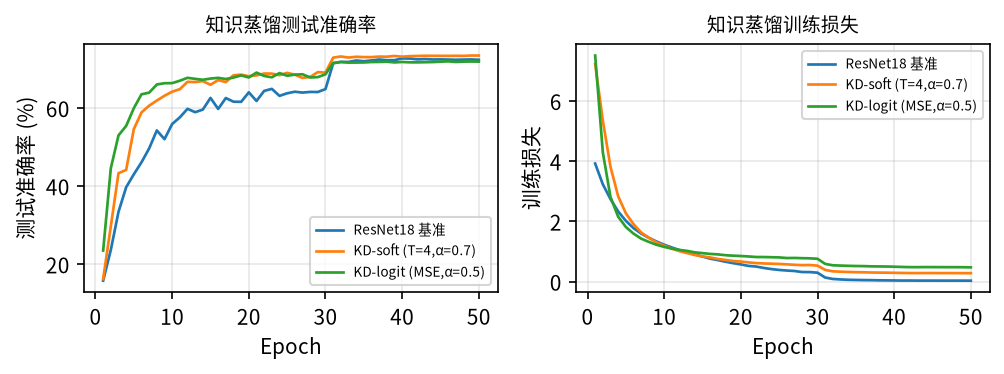
\includegraphics[width=0.8\textwidth]{../results/figs/fig5_kd.png}
  \caption{两种蒸馏损失对学生 ResNet18 的精度与收敛影响}\label{fig:kd}
\end{figure}

\subsection{结果分析}
soft target 的学生精度为 73.46\%，比无蒸馏基线高 0.73 点，且前期学得更快：
第 10 epoch 已经 64.20\%，基线同期只有 55.92\%。这一组的训练损失里含有蒸馏项
（第 1 epoch 就达到 7.2，约为 $0.3\,\mathcal{L}_{\text{CE}}+0.7\,T^2\mathrm{KL}$），
与纯交叉熵的数值不可直接比较，因此以精度曲线作为判据。

logits 对齐为 71.97\%，比基线低 0.76 点。该损失初期收敛很快，第 10 epoch 已达 66.39\%，之后增速下降。
可能的原因是 MSE 要求学生逐维贴合教师的 logit 数值，而 100 类分类中教师的 logit 尺度较大，
该项会将学生拉向教师的数值范围，后期优化难度较大，稳定性不如带温度的 KL。

实验中教师精度为 70.16\%，低于不蒸馏的学生基线，蒸馏后的学生比教师高 3.30 点。
教师是在 50 epoch 预算内未充分收敛的 ResNet50，但其输出仍包含类与类之间的相似性信息，
软标签为学生提供了额外约束，起正则化作用。据此，蒸馏的收益不完全取决于教师的绝对精度，
但更强的教师一般更有利。推理时只使用学生，11.2\,M 参数，约为教师的 47\%，
与普通 ResNet18 的部署开销相同。

$\alpha$ 取值过大时损失退化为普通交叉熵，过小时易受教师错误影响；本实验采用的 0.7 与 0.5
均较为稳定。$T$ 在 2 到 8 之间差别不大，$T=4$ 时软标签的信息量与锐度较为均衡。

% ------------------------------------------------------------------ 7
\section{任务 6：交通标志数据集分类与调参}
\begin{figure}[!htbp]
  \centering
  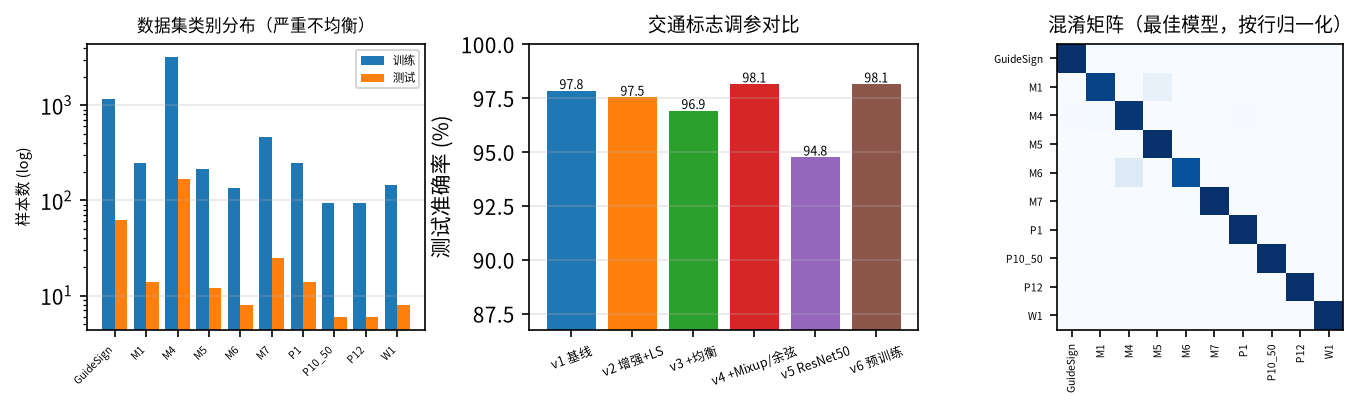
\includegraphics[width=0.95\textwidth]{../results/figs/fig6_traffic.png}
  \caption{交通标志数据集分布、六种方案精度对比与最佳模型混淆矩阵}\label{fig:traffic}

  \vspace{1pt}
  \captionof{table}{交通标志数据集上的 6 组调参方案}\label{tab:traffic}
  {\scriptsize
  \setlength{\tabcolsep}{0.5pt}
  \begin{tabular}{@{}L{1.9cm}*{6}{>{\centering\arraybackslash}p{1.55cm}}L{1.5cm}@{}}
  \toprule
  \thd{方案} & \makecell{\thd{数据}\\\thd{增强}} & \makecell{\thd{标签}\\\thd{平滑}} & \thd{采样} & \thd{epoch} & \makecell{\thd{最佳}\\\thd{精度(\%)}} & \makecell{\thd{耗时}\\\thd{(min)}}\\
  \midrule
  v1 基线 & Resize 128+CE & — & shuffle & 50 & 97.84 & 21.6\\
  v2 增强+LS & {\tiny\makecell[l]{Random\\ResizedCrop\\+Color\\Jitter\\+Rotation}} & 0.1 & shuffle & 50 & 97.53 & 25.8\\
  v3 +均衡采样 & 同 v2 & 0.1 & WRS & 50 & 96.91 & 24.3\\
  v4 +Mixup+余弦 & 同 v2 + Mixup($\alpha$=0.2) & 0.1 & WRS & 80 & 98.15 & 36.2\\
  v5 ResNet50(96) & 同 v4 & 0.1 & WRS & 40 & 94.75 & 31.0\\
  v6 预训练微调 & 同 v3 & 0.1 & WRS & 40 & \hl{98.15} & 2.0\\
  \bottomrule
  \end{tabular}
  \par\vspace{2pt}{\noindent\scriptsize 注：CE 为交叉熵损失，LS 为标签平滑 0.1，WRS 为 WeightedRandomSampler 均衡采样。}
  }
\end{figure}

\subsection{完成过程}
数据集共 10 类，训练 6024 张、测试 324 张，原始分辨率 224$\times$224，类别分布不均衡：
M4 有 3206 张，P10\_50 只有 95 张，测试集里最少的类只有 6 张（图~\ref{fig:traffic} 左）。

原来的接口是按 CIFAR 写的，这里重写了 Dataset。它遍历 train 与 test 下以类别命名的目录，
建立类别到索引的映射，读图后按统一的尺寸和归一化参数变换，返回张量与标签；
训练集与测试集走两条不同的变换流程，测试集只做缩放。
数据加载部分在标准 DataLoader 之外加了自定义采样器：训练集可以选随机打乱，也可以按类别频率加权，
权重取类样本数的倒数，batch 大小、worker 数与锁页内存都按本机设置；测试集按顺序加载，保证评估可复现。
归一化用的均值与标准差由训练集统计得到，存在结果目录里，均值约为 $[0.30, 0.39, 0.60]$。
训练增强包括随机缩放裁剪（0.7$\sim$1.0）、颜色抖动与 $\pm10^\circ$ 旋转；
交通标志水平翻转后会左右颠倒，因此未采用该增强。

调参按 6 组逐级叠加：v1 是基线，只做 Resize 128 和随机打乱，SGD lr=0.05 加 step 衰减；
v2 加强增强并加入标签平滑 0.1；v3 在 v2 基础上加类别均衡采样；
v4 在 v3 基础上去掉 step 换成余弦退火，再加 Mixup($\alpha$=0.2)，训练 80 epoch；
v5 换成 ResNet50，8\,GB 显存不足以使用原分辨率，改为 96$\times$96、batch=16、lr=0.03，训练 40 epoch；
v6 改用 ImageNet 预训练的 ResNet18，lr=0.005，微调 40 epoch，采样方式同 v3。
各组精度与耗时见表~\ref{tab:traffic}。


\subsection{结果分析}
v1 的 97.84\% 说明在这个数据集上，ResNet18 直接监督训练即可获得较高的精度：类别之间区别明显，
多数类的样本也充足。

v2 为 97.53\%，与 v1 只差一张测试图，总精度上看不出优势，但各类召回更均匀：宏平均召回由 94.58\% 升到
95.72\%，M1 由 71.4\% 升到 78.6\%，M6 由 75.0\% 升到 87.5\%。也就是说，增强与标签平滑针对的是弱类，
并没有去提高总体均值。

v3 的整体精度为 96.91\%，比 v2 低 0.62 点，宏平均 96.80\%，比 v2 高 1.08 点。M1 与 P1 继续上升，
但占测试集 52\% 的 M4 略有下降，总数被多数类拉着走低。这一组的结果正好说明，只报总体精度会掩盖
少数类上的变化。

v4 达到 98.15\%，是六组里从零训练的最高精度。与 v3 相比，它在 Mixup 之外把 step 换成了余弦退火，
epoch 增加到 80，决策边界因此更平滑。v5 为 94.75\%，比 v4 低 3.40 点，即使把分辨率降到 96$\times$96，
单 epoch 的耗时与 v4 相差也不大。本实验的训练集只有 6024 张，ResNet50 的容量用不满，加深网络没有收益。

v6 同为 98.15\%，耗时 2.0 min，约为 v4 的十八分之一。它和 v4 的正确数都是 318/324，
M1、M4、M6 的召回也相同，均为 92.9\%、97.6\%、87.5\%，区别只在于错的是哪几张图；宏平均为 97.80\%。
在训练样本有限的情况下，直接用 ImageNet 预训练权重比从零训练更省时间。

需要补充的是，测试集只有 324 张，错一张就是 0.31 点，P10\_50 只有 6 张，错一张即 16.7 点。
因此各组之间 1 点以内的差异不足以说明方法优劣，判断时还应结合宏平均召回和混淆矩阵。
\end{document}
